\documentclass[11pt]{article}
\usepackage{amssymb}
\usepackage{amsfonts}
\usepackage{amsmath}
\usepackage{bm}
\usepackage{latexsym}
\usepackage{epsfig}

\usepackage{tikz} % For drawing pictures. Used: environment "tikzpicture"

\setlength{\evensidemargin}{.25in}
\setlength{\textwidth}{6in}
\setlength{\topmargin}{-0.4in}
\setlength{\textheight}{8.5in}


\newcommand{\handout}[5]{
   \renewcommand{\thepage}{#1-\arabic{page}}
   \noindent
   \begin{center}
   \framebox{
      \vbox{
    \hbox to 5.78in {{\sf 18.312: Algebraic Combinatorics} 
\hfill \sf #2 }
       \vspace{4mm}
       \hbox to 5.78in { {\Large \hfill #5  \hfill} }
       \vspace{2mm}
       \hbox to 5.78in { {\em #3 \hfill #4} }
      }
   }
   \end{center}
   \vspace*{4mm}
}

\newcommand{\lecture}[4]{\handout{#1}{#2}{Lecture date: #3}{Notes by: #4}{Lecture #1}}


\textwidth=6in
\oddsidemargin=0.25in
\evensidemargin=0.25in
\topmargin=-0.1in
\footskip=0.8in
\parindent=0.0cm
\parskip=0.3cm
\textheight=8.00in
\setcounter{tocdepth} {3}
\setcounter{secnumdepth} {2}
\sloppy

\newtheorem{theorem}{Theorem}
\newtheorem{lemma}[theorem]{Lemma}
\newtheorem{proposition}[theorem]{Proposition}
\newtheorem{corollary}[theorem]{Corollary}
\newtheorem{fact}[theorem]{Fact}
\newtheorem{definition}[theorem]{Definition}
\newtheorem{remark}[theorem]{Remark}
\newtheorem{conjecture}[theorem]{Conjecture}
\newtheorem{question}[theorem]{Question}
\newtheorem{answer}[theorem]{Answer}
\newtheorem{exercise}[theorem]{Exercise}
\newtheorem{example}[theorem]{Example}
\newenvironment{proof}{\noindent \textbf{Proof:}}{$\Box$}

\newcommand{\N}{\mathbb N} % natural numbers 0,1,2,...
\newcommand{\Z}{\mathbb Z}  % integers
\newcommand{\R}{\mathbb R} % reals
\newcommand{\C}{\mathbb C} % complex numbers
\newcommand{\F}{\mathbb F} % finite fields

\newcommand{\floor}[1]{\left\lfloor {#1} \right\rfloor} % floor function
\newcommand{\ceiling}[1]{\left\lceil {#1} \right\rceil} % ceiling function
\newcommand{\binomial}[2]{\left( \begin{array}{c} {#1} \\ 
                        {#2} \end{array} \right)} % binomial coefficients
\newcommand{\modulo}[1]{\quad (\mbox{mod }{#1})} %congruences

\newcommand{\ignore}[1]{} % useful for commenting things out



% Shortcuts added for lecture 7
\newcommand{\keyword}[1]{{\emph{#1}}}
\newcommand{\intposet}[1]{{\mathbf{#1}}}

\begin{document}
\lecture{7}{Lionel Levine}{Feb 24, 2011}{Andrew Geng}
% replace n in the line above (and in the file name) by an actual integer
% replace Feb 1 by the date of the lecture 

\section{Partially ordered sets}

\subsection{Definitions}

\begin{definition}
    A \keyword{partially ordered set} (\keyword{poset} for short) is a set $P$
    with a binary relation $R \subseteq P \times P$ satisfying all of the
    following conditions.
    \begin{enumerate}
        \item (reflexivity) $(x,x) \in R$ for all $x \in P$
        \item (antisymmetry) $(x,y) \in R$ and $(y,x) \in R \  \Rightarrow \  x = y$
        \item (transitivity) $(x,y) \in R$ and $(y,z) \in R \  \Rightarrow \  (x,z) \in R$
    \end{enumerate}
\end{definition}
In analogy with the order on the integers by size, we will write
$(x,y) \in R$ as $x \leq y$ (or equivalently, $y \geq x$).
We will use $x < y$ to mean that $x \leq y$ and $x \neq y$.
When there are multiple posets in play, we can disambiguate by using
the name of the poset as a subscript, e.g. $x \leq_P y$.
\begin{remark}
    The word ``partial'' indicates that there's no guarantee that all elements
    can be compared to each other---i.e. we don't know that for all $x,y \in P$,
    at least one of $x \leq y$ and $x \geq y$ holds. A poset in which this
    is guaranteed is called a \keyword{totally ordered set}.
\end{remark}

Partially ordered sets can be visualized via \keyword{Hasse diagrams},
which we now proceed to define.
\begin{definition}
    Given $x, y$ in a poset $P$, the \keyword{interval} $[x,y]$ is the poset
    $\left\{z \in P \mid x \leq z \leq y\right\}$ with the same order as $P$.
\end{definition}
\begin{definition}
    ``$y$ \keyword{covers} $x$'' means $[x,y] = \{x,y\}$.
    That is, no elements of the poset lie strictly between $x$ and $y$
    (and $x \neq y$).
\end{definition}
\begin{definition}
    The \keyword{Hasse diagram} of a partially ordered set $P$ is the (directed)
    graph whose vertices are the elements of $P$ and whose edges are the pairs
    $(x,y)$ for which $y$ covers $x$. It is usually drawn so that elements
    are placed higher than the elements they cover.
\end{definition}

\subsection{Examples}

\begin{enumerate}
    \item
    $\intposet{n}$ (handwritten as $\underline{n}$) is the set $[n]$
    with the usual order on integers.
    \item
    The \keyword{Boolean algebra} $B_n$ is the set of subsets of $[n]$,
    ordered by inclusion. ($S \leq T$ means $S \subseteq T$).
\begin{figure}[ht]
    \caption{Hasse diagrams of $B_2$ and $B_3$}
    \begin{center}
    \begin{tikzpicture}
        \tikzstyle{every node} = [rectangle]
        \node (name) at (0,-1) {$B_2$};
        \node (s) at (0,0) {$\emptyset$};
        \node (s1) at (-1,1) {$\{1\}$};
        \node (s2) at (1,1) {$\{2\}$};
        \node (s12) at (0,2) {$\{1,2\}$};
        \foreach \from/\to in {s/s1, s/s2, s1/s12, s2/s12}
            \draw[->] (\from) -- (\to);
    \end{tikzpicture}
    \qquad
    \begin{tikzpicture}
        \tikzstyle{every node} = [rectangle]
        \node (name) at (0,-1) {$B_3$};
        \node (s) at (0,0) {$\emptyset$};
        \node (s1) at (-1,1) {$\{1\}$};
        \node (s2) at (0,1) {$\{2\}$};
        \node (s3) at (1,1) {$\{3\}$};
        \node (s23) at (-1,2) {$\{2,3\}$};
        \node (s13) at (0,2) {$\{1,3\}$};
        \node (s12) at (1,2) {$\{1,2\}$};
        \node (s123) at (0,3) {$\{1,2,3\}$};
        \foreach \from/\to in {s/s1, s/s2, s/s3,
                s2/s23, s3/s23, s1/s13, s3/s13, s1/s12, s2/s12,
                s23/s123, s13/s123, s12/s123}
            \draw[->] (\from) -- (\to);
    \end{tikzpicture}
    \end{center}
\end{figure}
\item
    $D_n = \{ \text{all divisors of } n\}$, with $d \leq d' \iff d \mid d'$.
\begin{figure}[ht]
    \caption{$D_{12} = \{1,2,3,4,6,12\}$}
    \begin{center}
    \begin{tikzpicture}
        \tikzstyle{every node} = [rectangle]
        \node (s1) at (0,0) {$1$};
        \node (s2) at (-1,1) {$2$};
        \node (s3) at (1,1) {$3$};
        \node (s4) at (-2,2) {$4$};
        \node (s6) at (0,2) {$6$};
        \node (s12) at (-1,3) {$12$};
        \foreach \from/\to in {s1/s2, s1/s3, s2/s4, s2/s6, s3/s6, s4/s12, s6/s12}
            \draw[->] (\from) -- (\to);
    \end{tikzpicture}
    \end{center}
\end{figure}
\item
    $\Pi_n = \{\text{partitions of } [n]\}$, ordered by refinement.
    \footnote{
        A \keyword{partition} of a set $X$ is a set of disjoint subsets of $X$
        whose union is $X$. We say that a partition $\sigma$ \keyword{refines}
        another partition $\tau$ (so, in the example, $\sigma \leq \tau$) if
        every $\sigma_i \in \sigma$ is a subset of some $\tau_{j(i)} \in \tau$.
    }
\item
    Generalizing $B_n$, any collection $P$ of subsets of a fixed set $X$
    is a partially ordered set ordered by inclusion.
    For instance, if $X$ is a vector space then we can take $P$
    to be the set of all linear subspaces. If $X$ is a group, we can take $P$
    to be the set of all subgroups or the set of all normal subgroups.
\end{enumerate}

\section{Maps between partially ordered sets}

\begin{definition}
    A function $f: P \to Q$ between partially ordered sets is \keyword{order-preserving}
    if $x \leq_P y \Rightarrow f(x) \leq_Q f(y)$.
\end{definition}
\begin{definition}
    Two partially ordered sets $P$ and $Q$ are \keyword{isomorphic} if
    there exists a bijective, order-preserving map between them whose inverse
    is also order-preserving.
\end{definition}
\begin{remark}
    For those familiar with topology, this should look like the definition
    of homeomorphic spaces---spaces linked by a continuous bijection whose
    inverse is also continuous. A continuous bijection can fail to have a
    continuous inverse if the topology of the domain has extra open sets;
    and an order-preserving bijection between posets can fail to have
    a continuous inverse if the codomain has extra order information.
\end{remark}

\subsection{Examples}

\begin{enumerate}
    \item $D_8 \simeq \intposet{4}$
    \item $D_6 \simeq B_2$
\end{enumerate}
\begin{figure}[ht]
    \caption{Hasse diagrams of isomorphic posets}
    \begin{center}
    \begin{tikzpicture}
        \tikzstyle{every node} = [rectangle]
        \node (name) at (0,-1) {$D_8$};
        \node (s1) at (0,0) {$1$};
        \node (s2) at (0,1) {$2$};
        \node (s3) at (0,2) {$4$};
        \node (s4) at (0,3) {$8$};
        \foreach \from/\to in {s1/s2, s2/s3, s3/s4}
            \draw[->] (\from) -- (\to);
    \end{tikzpicture}
    \quad
    \begin{tikzpicture}
        \tikzstyle{every node} = [rectangle]
        \node (name) at (0,-1) {$\intposet{4}$};
        \node (s1) at (0,0) {$1$};
        \node (s2) at (0,1) {$2$};
        \node (s3) at (0,2) {$3$};
        \node (s4) at (0,3) {$4$};
        \foreach \from/\to in {s1/s2, s2/s3, s3/s4}
            \draw[->] (\from) -- (\to);
    \end{tikzpicture}
    \qquad \qquad
    \begin{tikzpicture}
        \tikzstyle{every node} = [rectangle]
        \node (name) at (0,-1) {$D_6$};
        \node (s) at (0,0) {$1$};
        \node (s1) at (-1,1) {$2$};
        \node (s2) at (1,1) {$3$};
        \node (s12) at (0,2) {$6$};
        \foreach \from/\to in {s/s1, s/s2, s1/s12, s2/s12}
            \draw[->] (\from) -- (\to);
    \end{tikzpicture}
    \quad
    \begin{tikzpicture}
        \tikzstyle{every node} = [rectangle]
        \node (name) at (0,-1) {$B_2$};
        \node (s) at (0,0) {$\emptyset$};
        \node (s1) at (-1,1) {$\{1\}$};
        \node (s2) at (1,1) {$\{2\}$};
        \node (s12) at (0,2) {$\{1,2\}$};
        \foreach \from/\to in {s/s1, s/s2, s1/s12, s2/s12}
            \draw[->] (\from) -- (\to);
    \end{tikzpicture}
    \end{center}
\end{figure}

\section{Operations on partially ordered sets}
Given two partially ordered sets $P$ and $Q$, we can define
new partially ordered sets in the following ways.
\begin{enumerate}
\item
(Disjoint union)
$P + Q$ is the disjoint union set $P \sqcup Q$,
where $x \leq_{P+Q} y$ if and only if one of the following conditions holds.
\begin{itemize}
    \item $x, y \in P$ and $x \leq_P y$
    \item $x, y \in Q$ and $x \leq_Q y$
\end{itemize}
The Hasse diagram of $P + Q$ consists of the Hasse diagrams of $P$ and $Q$,
drawn together.
\item
(Ordinal sum)
$P \oplus Q$ is the set $P \sqcup Q$,
where $x \leq_{P \oplus Q} y$ if and only if one of the following conditions holds.
\begin{itemize}
    \item $x \leq_{P+Q} y$
    \item $x \in P$ and $y \in Q$
\end{itemize}
Note that the ordinal sum operation is not commutative. In $P \oplus Q$,
everything in $P$ is less than everything in $Q$.
\item
(Cartesian product)
$P \times Q$ is the Cartesian product set, $\left\{ (x,y) \mid x \in P, y \in Q \right\}$,
where $(x,y) \leq_{P \times Q} (x',y')$ if and only if both $x \leq_P x'$ and $y \leq_Q y'$.

The Hasse diagram of $P \times Q$ is the Cartesian product of the Hasse diagrams
of $P$ and $Q$.
\begin{example}
    $B_n \simeq \underbrace{\intposet{2} \times \cdots \times \intposet{2}}_{n \text{ times}}$
\end{example}
\begin{proof}
    Define a candidate isomorphism
    \begin{align*}
        f: \intposet{2} \times \cdots \times \intposet{2} &\to B_n \\
            (b_1, \cdots, b_n) &\mapsto \left\{ i \in [n] \mid b_i = 2 \right\} .
    \end{align*}
    It's easy to show that $f$ is bijective. To check that $f$ and $f^{-1}$
    are order-preserving, just observe that each of the following conditions
    is equivalent to the ones that come before and after it.
    \begin{itemize}
        \item $(b_1,\cdots,b_n) \leq (b_1', \cdots, b_n')$
        \item $b_i \leq b_i'$ for all $i$
        \item $\{ i \mid b_i = 2 \} \subseteq \{ i \mid b_i' = 2 \}$
        \item $f((b_1,\cdots,b_n)) \leq f((b_1',\cdots,b_n'))$
    \end{itemize}
\end{proof}
\begin{example}
    \label{lecturesevendistinctprimes}
    If $k = p_1 \cdots p_n$ is a product of $n$ distinct primes,
    then $D_k \simeq B_n$.
\end{example}
The proof of Example \ref{lecturesevendistinctprimes} is similarly easy,
using the isomorphism $f: D_k \to B_n$ defined by $\prod_{i \in S} p_i \mapsto S$.
\item
$P^Q$ is the set of order-preserving maps from $Q$ to $P$,
where $f \leq_{P^Q} g$ means that $f(x) \leq_P g(x)$ for all $x \in Q$.

The notation $P^Q$ can be motivated by a basic example.
\begin{example}
\begin{align*}
    P &= \overbrace{\intposet{1} + \cdots + \intposet{1}}^n \\
    Q &= \overbrace{\intposet{1} + \cdots + \intposet{1}}^k \\
    P^Q &\simeq \overbrace{\intposet{1} + \cdots + \intposet{1}}^{n^k}
\end{align*}
\end{example}
Perhaps more importantly, the following properties hold
(the proof is the 15th homework problem).
\begin{align*}
    P^{Q + R} &\simeq P^Q \times P^R \\
    \left(P^Q\right)^R &\simeq P^{Q \times R}
\end{align*}

\begin{example}
    The partially ordered set $\intposet{2}^\intposet{2}$ is isomorphic to $\intposet{3}$.
\end{example}
\begin{proof}
    The order-preserving
    maps are specified by $f_1(1) = f_1(2) = 1$, $f_2 = id$, and
    $f_3(1) = f_3(2) = 2$; so $f_1 \leq f_2 \leq f_3$.
\end{proof}
\end{enumerate}

\section{Graded posets}

\begin{definition}
    A \keyword{chain} of a partially ordered set $P$ is a totally ordered subset
    $C \subseteq P$---i.e. $C = \{ x_0, \cdots, x_\ell \}$ with
    $x_0 \leq \cdots \leq x_\ell$. The quantity $\ell = |C| - 1$ is its
    \keyword{length} and is equal to the number of edges in its Hasse diagram.
\end{definition}
\begin{definition}
    A chain is \keyword{maximal} if no other chain strictly contains it.
\end{definition}
\begin{definition}
    The \keyword{rank} of $P$ is the length of the longest chain in $P$.
\end{definition}
\begin{definition}
    $P$ is \keyword{graded} if all maximal chains have the same length.
\end{definition}
\begin{figure}[ht]
    \caption{Hasse diagram of a poset that is not graded}
    \begin{center}
    \begin{tikzpicture}
        \tikzstyle{every node} = [draw, shape=circle]
        \node (s1) at (0,0) {};
        \node (s2) at (-1,1) {};
        \node (s3) at (-1,2) {};
        \node (s4) at (0,3) {};
        \node (sx) at (1,1.5) {};
        \foreach \from/\to in {s1/s2, s2/s3, s3/s4, s1/sx, sx/s4}
            \draw[->] (\from) -- (\to);
    \end{tikzpicture}
    \end{center}
\end{figure}
\begin{definition}
    A \keyword{rank function} on a poset $P$ is a map $r: P \to \{0,\cdots,n\}$
    for some $n$, satisfying the following properties.
    \begin{enumerate}
        \item $r(x) = 0$ for all minimal $x$ (i.e. there is no $y < x$).
        \item $r(x) = n$ for all maximal $x$.
        \item $r(y) = r(x) + 1$ whenever $y$ covers $x$.
    \end{enumerate}
\end{definition}

\begin{lemma}
    $P$ is graded of rank $n$ $\iff$ there exists a rank function
    $r: P \to \{0,\cdots,n\}$.
\end{lemma}
\begin{example}
    $B_n$ is graded, and cardinality is a rank function on $B_n$.
\end{example}
\begin{proof}
    \begin{itemize}
        \item[$\Rightarrow$ :]
            If $P$ is graded of rank $n$, define
            $r(x) = \#\{ y \in C \mid y < x \}$
            where $C$ is a maximal chain containing $x$. To check that this is
            well-defined, we need to show that it is independent of $C$.

            So suppose $C$ and $C'$ are maximal chains containing $x$.  Write
            \begin{align*}
                C &= C_0 \sqcup \{x\} \sqcup C_1 \\
                C' &= C'_0 \sqcup \{x\} \sqcup C'_1
            \end{align*}
            where $C_0 = \{y \in C \mid y<x\}$ and $C'_0 = \{y \in C' \mid y<x\}$.
            If $|C_0| \neq |C'_0|$, then assuming without loss of generality
            that $|C_0| > |C'_0|$, the chain $C_0 \cup x \cup C'_1$
            would have length greater than $n$. $P$ being graded of rank $n$
            disallows this, so $|C_0| = |C'_0| = r(x)$.

            This establishes that $r(x)$ is well-defined.
            It is easy to see by maximality of the chains involved
            that $r$ is indeed a rank function.
        \item[$\Leftarrow$ :]
            Given a rank function $r: P \to \{0,\cdots,n\}$
            and a maximal chain $C = \{x_0,\cdots,x_\ell\}$, we observe that
            \begin{itemize}
                \item $x_0$ is minimal (otherwise $C$ could be extended by
                    anything less than $x_0$),
                \item $x_\ell$ is maximal (otherwise $C$ could be extended
                    by anything greater than $x_\ell$), and
                \item $x_{i+1}$ covers $x_i$ (otherwise the element between
                    them could be inserted into $C$).
            \end{itemize}
            Then $r(x_0) = 0$, $r(x_\ell) = n$, and $r(x_{i+1}) = r(x_i) + 1$ for $i=0,1,\ldots,\ell-1$,
            so we see that $\ell = n$.
    \end{itemize}
\end{proof}
\begin{remark}
    If a rank function exists, it is in fact uniquely defined.
\end{remark}
\begin{corollary}
    Any interval in a graded poset is graded.
\end{corollary}
\begin{proof}
    For $[x,y] \subset P$, use the rank function $r_{[x,y]}(z) = r_P(z) - r_P(x)$.
\end{proof}

\section{Lattices}

\begin{definition}
    A poset $L$ is a \keyword{lattice} if every pair of elements $x,y$ has
    \begin{itemize}
        \item a \keyword{least upper bound} $x \vee y$ (a.k.a. \keyword{join}), and
        \item a \keyword{greatest lower bound} $x \wedge y$ (a.k.a. \keyword{meet});
    \end{itemize}
    i.e.
    \begin{align*}
        z \geq x \vee y &\iff z \geq x \text{ and } z \geq y \\
        z \leq x \wedge y &\iff z \leq x \text{ and } z \leq y .
    \end{align*}
\end{definition}
\begin{example}
    $B_n$ is a lattice. The meet and join can be explicitly specified as
    \begin{align*}
        S \cap T &= S \wedge T
        &
        S \cup T &= S \vee T ,
    \end{align*}
    and this can serve as a mnemonic for the symbols.
\end{example}

\begin{figure}[ht]
    \caption{Hasse diagram of part of a lattice}
    \begin{center}
    \begin{tikzpicture}
        \tikzstyle{every node} = [rectangle]
        \node (s) at (0,0) {$x \wedge y$};
        \node (s1) at (-1,1) {$x$};
        \node (s2) at (1,1) {$y$};
        \node (s12) at (0,2) {$x \vee y$};
        \foreach \from/\to in {s/s1, s/s2, s1/s12, s2/s12}
            \draw[->] (\from) -- (\to);
    \end{tikzpicture}
    \end{center}
\end{figure}

\end{document}
